% !TEX root = main.tex
\chapter{Introduzione}
Nel progetto sono stati affrontati alcuni dei vari problemi che riguardano l'intelligenza artificiale. In questa relazione spiegheremo quali soluzioni sono state adottate, i vantaggi e gli svantaggi e alcuni miglioramenti che possono esser fatti al nostro progetto

\section{Strategie}
Per svolgere il progetto di IA-LAB sono state implementate 4 strategie in maniera incrementale:
\begin{itemize}
  \item FIFO WAIT: la strategia usa la politica fifo come politica di scelta degli ordini. 
  \item FIFO: Simile alla precendente, ma in caso di ostacolo che non permette di servire un ordine, l'ordine viene messo al fondo.
  \item LOW PENALITY: strategia che si basa sulla penalità per effettuare la scelta dell'ordine.
  \item HARD: a differenza delle altre 3 strategia, questa permette di gestire più ordini in contemporanea. Come la precedente si basa sulle penalità.
\end{itemize}

Ogni strategia è stata suddivisa in fasi dove ogni fase si occupa di uno specifico sotto-problema. Questa suddivisione ci ha permesso sia uno sviluppo incrementale all'interno della stessa strategia, sia tra strategie diverse, dove è bastato andare a sviluppare in modo più articolato una fase oppure nell'inserire nuove fasi.

\subsection{Astar}
Tutte le strategia utilizzano il modulo Astar per pianificare dei piani che permettano al nostro robot di spostarsi da un punto A a un punto B. Il punto A è la posizione del robot al momento della pianificazione mentre il goal (il punto B) è dato dalla cella destinazione. La cella destinazione può essere un dispenser, un cestino o un tavolo. Il modulo astar calcolerà quali sono i 4 punti di accesso alla nostra destinazione e si fermerà non appena arriverà a uno di esso.

Il modulo A* può terminare fornendo un piano, oppure può fallire. Per memorizzare il piano creato vengono usate due strutture:

\begin{lstlisting}
(deftemplate plane 
	(slot plane-id) 
	(multislot pos-start) 
	(multislot pos-end) 
	(slot direction) 
	(slot cost) 
	(slot status (allowed-values ok failure))
)
\end{lstlisting}
\begin{lstlisting}
(deftemplate step-plane 
	(slot plane-id)
	(slot action)
	(slot direction)
	(multislot pos-start)
	(slot father)
	(slot child)
)
\end{lstlisting}

La struttura step-plane indica i vari passi per eseguire il piano plane. I piani vengono memorizzati in modo tale che il robot non debba ripianificare più volte uno stesso percorso. Vengono memorizzati solo i piani principali; nel caso in cui un piano fallisca il piano "riparatore" non viene memorizzato.

\chapter{Strategie}
\section{Strategia FIFO WAIT}
La prima strategia che illuestreremo è la FIFO WAIT. \'E una strategia molto semplice, dove il primo ordine che arriva è l'ordine che viene servito. Vi sono vari casi per completare un ordine:\begin{itemize}
  \item Ordine Accepted: un ordine di questo tipo verrà completato solo quando verranno consegnate al tavolo tutte le consumazioni richieste.
  \item Ordine Delayed: un ordine di questo tipo verrà completato solo quando verranno consegnate al tavolo tutte le consumazioni richieste. Rispetto al caso precedente le consumazioni non potranno esser consengate fin quando il tavolo non sarà finito.
  \item Ordine Finish: un ordine di questo tipo verrà completato solo quanto verrà pulito il tavolo e il robot butterà lo sporco nei vari cestini.
\end{itemize}

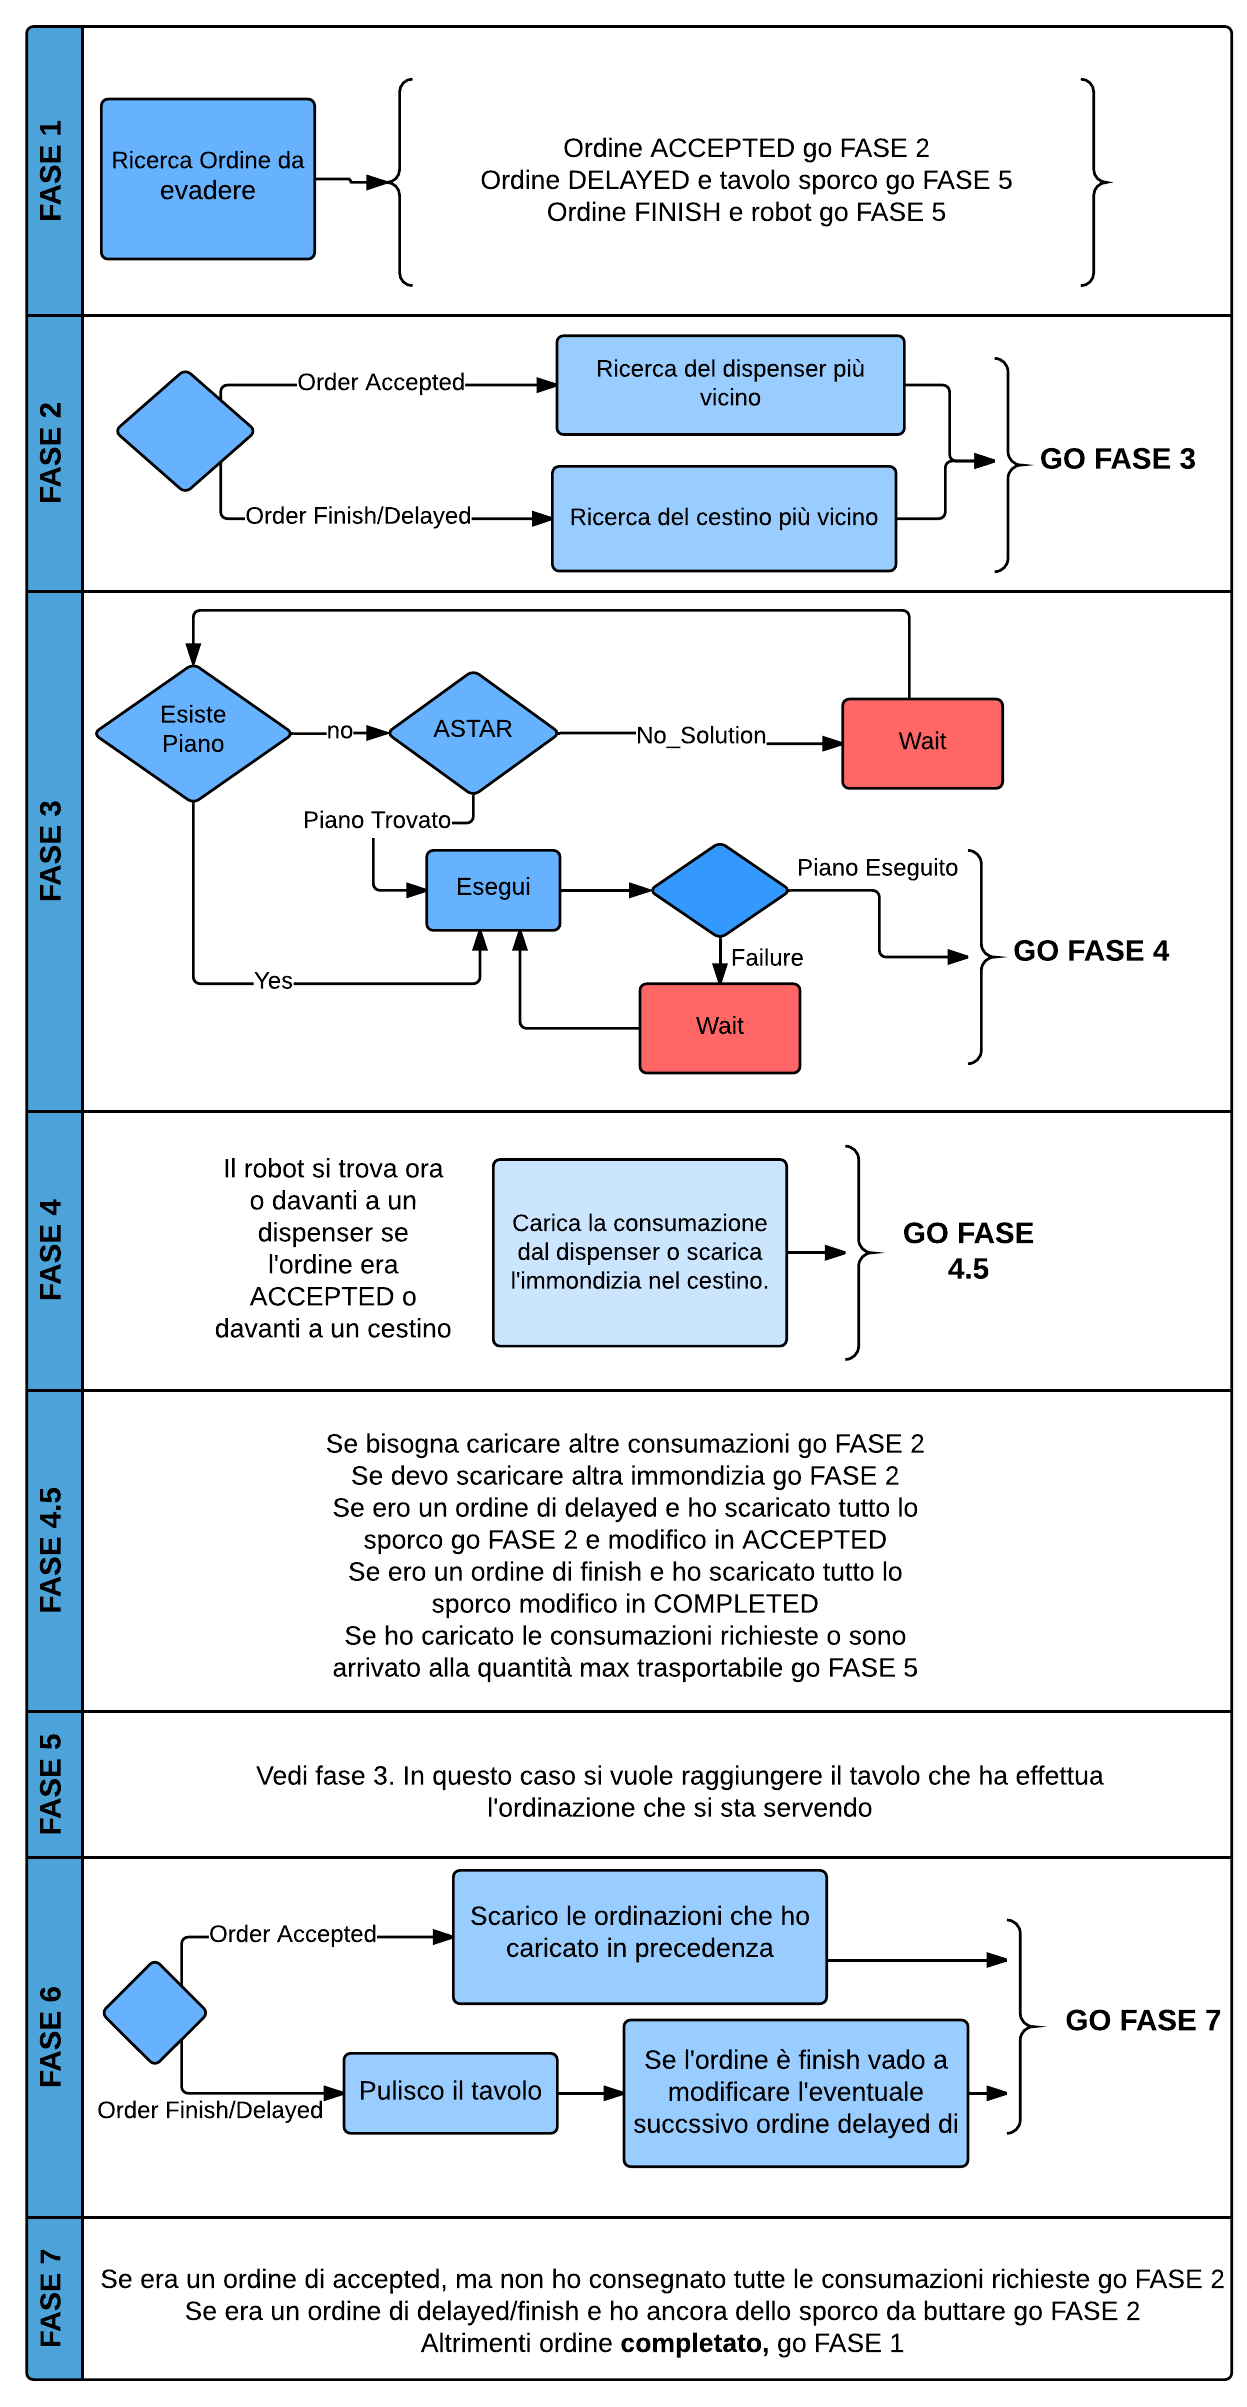
\includegraphics[width=\textwidth]{schema-fifo-wait.png}